% Chapter 2

\chapter{Como Usar o \textit{Template} \LaTeX{} para Relatórios de PESTA}	%The main chapter title
\chaptermark{O \textit{Template}}	%Short version for page header. Comment if not needed
\label{Chapter2}	%For referencing the chapter elsewhere, use \ref{Chapter2} 

%%%%%%%%%%%%%%%%%%%%%%%%%%%%%%%%%%%%

A opção pelo \LaTeX{} para elaborar o relatório favorece o aspeto gráfico do documento final, mas um documento visualmente bonito não substitui uma escrita cuidada e com uma apresentação de ideias estruturada. O presente capitulo é dedicado a apresentar o \textit{template} e alguns aspetos de como inserir citações, figuras, tabelas, equações e outros elementos cuja formatação deverá ser consistente ao longo de todo o documento.

O \textit{template} \LaTeX{} para relatórios da \ac{leec} e da \ac{leti} foi desenvolvido, e é mantido, por Vitor Cunha, baseado no \textit{template} ``Masters/Doctoral Thesis'' disponível em \url{www.LaTeXTemplates.com}. Sugestões e comentários podem ser enviados para \verb|vrc@isep.ipp.pt|. No entanto salienta-se que, \underline{o \textit{template} é fornecido sem suporte} e que é da inteira responsabilidade do utilizador qualquer alteração ao código e/ou ficheiros fornecidos.

\begin{comment}
The comment environment is used to easily comment large sections of LateX code. The comment environment is used to easily comment large sections of LateX code. The comment environment is used to easily comment large sections of LateX code. The comment environment is used to easily comment large sections of LateX code. The comment environment is used to easily comment large sections of LateX code.
\end{comment}

%%%%%%%%%%%%%%%%%%%%%%%%%%%%%%%%%%%%

\section{Introdução ao \LaTeX{}}
\label{sec:Ch2.1}

O \LaTeX{} é uma poderosa ferramenta para produção de documentos. Ao contrário dos comuns processadores de texto como o Microsoft Word ou o LibreOffice Writer, o \LaTeX{} não é um programa \ac{wys}. Em vez disso, um documento escrito para \LaTeX{} é na verdade um simples ficheiro de texto sem qualquer tipo de formatação. Qualquer formato que se pretenda no documento final é definido através de comandos específicos que o \LaTeX{} interpreta aquando da compilação do documento. Por exemplo, para colocar uma palavra em itálico, no ficheiro de código escreve-se \verb|\textit{palavra}| para obter \textit{palavra} no documento final. Isso significa que o \LaTeX{} é uma linguagem \emph{markup}, à semelhança do \ac{html}. Desta forma o autor pode centrar-se na tarefa essencial da escrita, sem ter que se preocupar com formatações, paginação e outros arranjos visuais do documento em preparação. O \LaTeX{} é amplamente utilizado no meio académico para a elaboração e publicação de documentos científicos em várias áreas, incluindo matemática, estatística, engenharia, física, economia, entre muitas outras. Tem também um importante papel na preparação e publicação de livros.

Para quem está a começar com o \LaTeX{}, para além dos inúmeros \textit{websites} com informação (e.g., \url{www.overleaf.com/learn}), recomenda-se o livro gratuito intitulado ``Uma não tão pequena introdução ao \LaTeX{}'' disponível em \url{ftp.eq.uc.pt/software/TeX/info/lshort/portuguese/pt-lshort.pdf}. Este livro está também disponível em vários idiomas em \url{www.ctan.org/tex-archive/info/lshort/}.

%%%%%%%%%%%%%%%%%%%%%%%%%%%%%%%%%%%%

\section{Como Usar o Template}

O \textit{template} encontra-se disponível e pronto a ser usado no Moodle e na \href{https://www.overleaf.com/latex/templates/isep-dee-bsc-latex-template/kqkmqnjbbpvj}{\textit{Overleaf Templates Gallery}}. Independentemente de optar por desenvolver o seu relatório no Overleaf ou localmente no seu computador pessoal, é indispensável a familiarização com a estrutura de diretórios e ficheiros fornecidos com o \textit{template}.

\subsection{Diretórios}

Os nomes dos diretórios são, geralmente, auto explicativos:

\begin{itemize}
     \item \textbf{chapters} -- este diretório é onde deverá colocar os capítulos do relatório, incluindo os anexos. Cada capítulo (e anexo) deve ter o seu próprio ficheiro \file{.tex} e, embora não haja nenhuma regra rígida para o nome e número de capítulos, terá que existir sempre uma ``Introdução'' e as ``Conclusões''.

     \item \textbf{figures} -- este diretório deverá conter todas as figuras usadas no relatório. Recomenda-se o uso de um sistema de nomes de ficheiros que facilite a associação de um ficheiro a uma secção do documento.

     \item \textbf{front} -- este diretório contém desde logo vários ficheiros destinados às secções iniciais pré-definidas do relatório, designadas de \textit{frontmatter}. Poderá optar por não usar algumas destas secções caso não sejam relevantes para o seu documento.
\end{itemize}

\subsection{Ficheiros}

Adicionalmente à estrutura de diretórios são também fornecidos vários ficheiros, a maioria deles em texto simples e cujo conteúdo pode ser visto com um editor de texto. Após a compilação com o \LaTeX{} vários ficheiros auxiliares são criados automaticamente, no entanto, regra geral, não necessita de os ter em consideração.

\begin{itemize}
\item \textbf{sampleRefs.bib} -- este é o ficheiro para o BibTeX que contém todas as referências que irá citar no relatório. Este pode ser editado manualmente, mas existem programas disponíveis (e.g., \url{www.jabref.org}) para gerir referências que facilitam todo o processo. Pode mudar o nome do ficheiro desde que essa alteração também seja feita no ficheiro \file{main.tex}. As referências serão apresentadas no documento final com o estilo \textbf{ieeetr}. Considere os exemplos de vários tipos de referências fornecidos no ficheiro \file{sampleRefs.bib} para elaborar a sua própria lista.

\item \textbf{DEEclass.cls} -- este ficheiro define a classe de documento DEEclass. É veementemente desaconselhado a sua modificação.

\item \textbf{preamble.tex} -- este ficheiro deverá ser usado para adicionar \glspl{pack}, configurações e macros, específicos do seu documento. Desta forma evita-se que o preâmbulo do ficheiro principal \file{main.tex} fique demasiado extenso. 

\item \textbf{main.tex} -- este é o ficheiro mais importante para a definição do seu documento. O código deste ficheiro define a estrutura e contém as instruções que levam o \LaTeX{} a gerar o PDF final. Tenha em consideração os comentários apresentados no próprio ficheiro por forma a saber o que faz cada linha/secção de código e de como o \textit{template} pode ser adaptado ao seu caso. É este ficheiro que deverá editar para dar como iniciada a elaboração do seu relatório. Parabéns por ter decidido usar o \LaTeX{}!
\end{itemize}

%%%%%%%%%%%%%%%%%%%%%%%%%%%%%%%%%%%%

\subsection{Edição do ficheiro \file{main.tex}}
\label{subsec:Ch2.2.3}

Para começar o seu documento, a primeira coisa a fazer é preencher as suas informações e escolher algumas opções no ficheiro \file{main.tex}. Depois de abrir este ficheiro, localize a secção identificada como ``MAIN SETTINGS'' (linha 18). Nesta secção deverá escolher o seu curso, das duas opções:

\begin{itemize}
\item \acs{leec} (\acl{leec})
\item \acs{leti} (\acl{leti})
\end{itemize}
\newpage
\noindent e o idioma principal do documento, das duas opções: 
\begin{itemize}
\item portuguese 
\item english
\end{itemize}

Ao escolher português como o idioma principal, é automaticamente usado como 2º o inglês. O oposto acontece se escolher inglês como idioma principal do documento. 

Para prosseguir com a personalização localize a secção ``REPORT INFORMATION'' (linha 29). Após preencher os campos desta secção com os dados:

\begin{itemize}
\item título do trabalho (e subtítulo se necessário),
\item identificação do candidato (nome, nº mecanográfico e \textit{email}),
\item identificação do orientador do \ac{isep} (nome e \textit{email}),
\item se aplicável, identificação do coorientador do \ac{isep} (nome e \textit{email}),
\item se aplicável, identificação da empresa onde decorreu o estágio (nome) e do orientador (nome e \textit{email}), 
\end{itemize}

\noindent pode compilar o seu documento. Todas as informações introduzidas devem estar agora visíveis (nas folhas de capa) no PDF gerado.

O ficheiro \file{main.tex} serve também para definir a estrutura e os conteúdos do relatório. Tenha em consideração os comentários que pode ler ao longo do ficheiro para saber onde colocar, e.g., novos capítulos ou ocultar secções que não pretenda usar no seu documento (e.g., ``Dedicatória''). De forma resumida na secção ``FRONTMATTER'' (linha 55):

\begin{itemize}
\item A linha \verb|%----------------------------------------------------------------------------------------
%	DEDICATION
%----------------------------------------------------------------------------------------

\dedicatory{
(Opcional) Poderá usar esta secção para dedicar o trabalho a alguém\ldots
} 
| refere-se à secção ``Dedicatória''. Se pretende escrever uma dedicatória edite o ficheiro \path{/front/1_dedicatory.tex}. Caso contrário basta comentar a linha para que o conteúdo do ficheiro não seja considerado.
\item A linha \verb|%---------------------------------------------------------
%	ACKNOWLEDGEMENTS
%---------------------------------------------------------
\begin{acknowledgements}
Ao \ac{isep}, como instituto com fortes valores e princípios, que permaneçam no bom caminho, criando cada vez mais formandos aptos para enfrentar os desafios do futuro, e crescer de forma positiva. Agradecer aos docentes que partilharam seus conhecimentos e nos permitiu desenvolver as competências necessárias para atingir os nossos objetivos. \\
\\
Um especial agradecimento ao orientador do Projeto/Estagio Engª Isabel Gonçalves Vaz, pelos conselhos e opiniões.
\end{acknowledgements}
%%%%%%%%%%%%%%%%%%%%%%%%%%%%%%%%%%%%%%%%%%%%%%%%%%%%%%%%%%
| refere-se à secção ``Agradecimentos'' e para a editar aceda ao ficheiro \path{/front/2_acknowledgements.tex}.
\item A linha \verb|%----------------------------------------------------------------------------------------
%	ABSTRACT PAGES
%----------------------------------------------------------------------------------------

% IMPORTANT NOTE: the abstract must always be written in two languages. If the report
% is written in Portuguese you have selected 'portuguese' as the language in the document class.
% Therefore, the portuguese version of the abstract must come first, so write it in the
% below area denoted by 'MAIN LANGUAGE ABSTRACT'. The english version follows in the
% 'SECOND LANGUAGE ABSTRACT' section.
% If the report is written in English, first will come the abstract in English
% ('MAIN LANGUAGE ABSTRACT') and then in Portuguese ('SECOND LANGUAGE ABSTRACT').

\begin{abstract}
%%%%%%%%%%%%%%%%%%%%%%%%%%%%%% MAIN LANGUAGE ABSTRACT %%%%%%%%%%%%%%%%%%%%%%%%%%%%%%%%%%

Aqui deverá ser apresentado o resumo de todo o trabalho efetuado. Esta secção não deverá exceder uma página.

Deve contextualizar o problema que pretende resolver ou a hipótese que irá formular, procure evidenciar as vantagens e desvantagens (se as houver) da solução encontrada, como também a forma através da qual a solução/hipótese foi validada. Neste último ponto, deverá referir-se aos desenvolvimentos efetuados, e à forma como validou (conformidade) e avaliou (desempenho) a solução encontrada.

O documento deve conter sempre duas versões do resumo: uma primeira no idioma do texto principal e a segunda num outro idioma. Este \textit{template} assume que os dois idiomas em consideração são sempre Português e Inglês, assim, a classe irá colocar os cabeçalhos respetivos de acordo com o idioma selecionado nas opções da classe no ficheiro \file{main.tex}. 

%----------------------------------------------------------------------------------------

\vspace*{10mm} 
\noindent
\textbf{\keywordslabel}: Lista, separada por vírgulas, de palavras, frases, ou acrónimos chave no âmbito do trabalho descrito neste texto. 

%%%%%%%%%%%%%%%%%%%%%%%%% END OF THE MAIN LANGUAGE ABSTRACT %%%%%%%%%%%%%%%%%%%%%%%%%%%%%%
\end{abstract}
\begin{secondlangabstract}
%%%%%%%%%%%%%%%%%%%%%%%%%%%%%% SECOND LANGUAGE ABSTRACT %%%%%%%%%%%%%%%%%%%%%%%%%%%%%%%%%%

The summary of all the developed work should be presented here. This section should not exceed one page.

Start the abstract with the contextualization of the problem you intend to solve or the hypothesis you will formulate. Try to highlight the advantages and disadvantages (if any) of the solution found, as well as the way in which the solution/hypothesis was validated. In this last point, you should refer to the developments made, and to the way you validated (compliance) and evaluated (performance) the solution found.

The document must always contain two versions of the abstract: a first in the language of the main text and the second one in another language. This template assumes that the two languages are always Portuguese and English, therefore, the class will place the correct section headers according to the language selected in the class options in the \file{main.tex} file.


%----------------------------------------------------------------------------------------

\vspace*{10mm} 
\noindent
\textbf{\keywordslabel}: Comma separated list of words, phrases, or key acronyms within the scope of your developed work. 

%%%%%%%%%%%%%%%%%%%%%%%%%% END OF THE SECOND LANGUAGE ABSTRACT %%%%%%%%%%%%%%%%%%%%%%%%%%%%%
\end{secondlangabstract}

| refere-se às secções ``Resumo'' e ``Abstract'', e o seu conteúdo é alterado no ficheiro \path{/front/3_abstract.tex}. Note que terá sempre que escrever esta secção em dois idiomas, leia atentamente as instruções contidas no ficheiro. É nesta secção onde também são introduzidas as palavras-chave associadas ao seu trabalho.
\item A linha \verb|%----------------------------------------------------------------------------------------
%	FONTMATTER LISTS
%----------------------------------------------------------------------------------------
\pdfbookmark[0]{\contentsname}{toc}
\tableofcontents 	
\glsresetall
%----------------------------------------------------------------------------------------

% Of the following lists, comment the ones you will not use in your document

\listoffigures 			% Prints the list of figures

\listoftables 			% Prints the list of tables

\printlistoflistings	% Prints the list of listings (source code segments)

\printlistofterms		% Prints the list of USED terms (glossary)

\printlistofacronyms{XXXXXXXXI} % Prints the list of USED acronyms
% Change the argument with random letters to adjust the left alignment of the acronyms full name column

\printlistofsymbols		% Prints the list of ALL defined symbols
| refere-se às secções ``Lista de Figuras'', ``Lista de Tabelas'', ``Listagens'', ``Glossário'', ``Lista de Acrónimos'' e ``Lista de Símbolos''. Deverá editar o conteúdo do ficheiro \path{/front/4_frontmatterlists.tex} para selecionar (comentando ou não as respetivas linhas) que secções deverão fazer parte do seu documento.
\end{itemize}

Qualquer uma das linhas pode ser comentada caso não queira usar a respetiva secção, a DEEclass trata de todos os aspetos de paginação e formatação do documento final. Para adicionar conteúdos às listas de termos, acrónimos e símbolos, localize a secção ``USER DEFINED LISTS'' (linha 45).

\begin{itemize}
\item A linha \verb|%---------------------------------------------------------
%	GLOSSARY
%---------------------------------------------------------
% Only the used entries will be displayed in the printed list, ie, you need to used a term at least once
% In italic if not in the main document language
% terms definition usage:
% \newglossaryentry{<tag>}{name={<term>},description={<description of the term>}}
%\makeglossaries
\newglossaryentry{gloss}{
name={glossário}, 
description={é uma lista alfabética de termos de um determinado domínio de conhecimento com a definição desses mesmos termos.},
}
\newglossaryentry{pack}{
name={\textit{package}}, 
description={é um ficheiro ou conjunto de ficheiros que contêm comandos \LaTeX{} extra que adicionam novas funcionalidades de estilo ou modificam aquelas já existentes.},
sort={package}	%needed for sorting when using LaTeX commands in the 'name' field
}
\newglossaryentry{lipsum}{
name={\textit{Lorem Ipsum}}, 
description={é uma sequência de palavras, geralmente latinas, utilizada para preencher o espaço destinado a texto numa publicação, por forma a testar as opções de formatação e edição e o arranjo dos elementos gráficos antes da inserção do conteúdo.},
sort={Lorem Ipsum}
}
%%%%%%%%%%%%%%%%%%%%%%%%%%%%%%%%%%%%%%%%%%%%%%%%%%%%%%%%%%%%%%%%
\newglossarystyle{mylong}{%
	\setglossarystyle{long}%
	\renewenvironment{theglossary}%
	{\begin{longtable}[l]{@{}p{\dimexpr 3cm-\tabcolsep}p{.7\hsize}}}% <-- change the value here
		{\end{longtable}}%
}
\newglossaryentry{latex}
{
	name=latex,
	description={Is a mark up language specially suited 
		for scientific documents}
}
\newglossaryentry{maths}
{
	name=mathematics,
	description={Mathematics is what mathematicians do}
}
\newglossaryentry{formula}{
	name=formula,
	description={A mathematical expression}
}
\newglossaryentry{Biofouling}{
	name=Biofouling,description={Some description}
}
\newglossaryentry{symb:Pi}{
	name=\ensuremath{\pi},
	description={Geometrical value}
}
%%%%%%%%%%%%%%%%%%%%%%%%%%%%%%%%%%%%%%%%%%%%%%%%%%%%%%%%%%
| refere-se às secções ``Glossário''. Edite o ficheiro \path{/front/0_glossary.tex} para elaborar o dicionário do seu relatório.
\item A linha \verb|%----------------------------------------------------------------------------------------
%	ACRONYMS LIST
%----------------------------------------------------------------------------------------

% Only the used entries will be displayed in the printed list, ie, you need to used a acronym at least once
% Full name in italic if not in the main document language

%acronym definition usage:
%\newacronym{<tag>}{<acronym>}{<full name>}

\newacronym{wys}{WYSIWYG}{\textit{What You See Is What You Get}}
\newacronym{dee}{DEE}{Departamento de Engenharia Electrotécnica}
\newacronym{api}{API}{\textit{Application Programming Interface}}
\newacronym{ascii}{ASCII}{\textit{American Standard Code for Information Interchange}}
\newacronym{html}{HTML}{\textit{HyperText Markup Language}}
\newacronym{isep}{ISEP}{Instituto Superior de Engenharia do Porto}
\newacronym{leec}{LEEC}{Licenciatura em Engenharia Eletrot\'{e}cnica e de Computadores}
\newacronym{leti}{LETI}{Licenciatura em Engenharia de Telecomunicações e Informática}
\newacronym{usb}{USB}{\textit{Universal Serial Bus}}
\newacronym{pdf}{PDF}{\textit{Portable Document Format}}
| refere-se à secção ``Lista de Acrónimos''. Edite o ficheiro \path{/front/5_listofacronyms.tex} para elaborar a sua lista de acrónimos.
\item No mesmo sentido, a linha \verb|%---------------------------------------------------------
%	SYMBOLS LIST
%---------------------------------------------------------
% terms definition usage:
% \newglossaryentry{<tag>}{
% name={<symbol>},
% sort={<text for the alphabetical sorting>},
% description={<description of the symbol>},
% unit={<units to display>},
% type=symbolslist}
\newglossaryentry{f}{
name={\ensuremath{f}},
sort={f},
description={força},
unit=\si{\newton},
type=symbolslist}
\newglossaryentry{i}{
name={\ensuremath{i}},
sort={i},
description={corrente},
unit=\si{\ampere},
type=symbolslist}
\newglossaryentry{m}{
name=\ensuremath{M},
sort={m},
description={massa},
unit=\si{\kilogram},
type=symbolslist}
\newglossaryentry{p}{
name=\ensuremath{P},
sort={p},
description={potência},
unit=\si{\watt},
type=symbolslist}
\newglossaryentry{theta}{
name=\ensuremath{\theta},
sort={z1},
description={deslocamento angular},
unit=\si{\radian},
type=symbolslist}
\newglossaryentry{omega}{
name=\ensuremath{\omega},
sort={z2},
description={velocidade angular},
unit=\si{\radian\per\second},
type=symbolslist}
\newglossaryentry{x}{
name=\ensuremath{x},
sort={x},
description={deslocamento},
unit=\si{\meter},
type=symbolslist}
% Greek: alpha,beta,gamma,delta,epsilon,zeta,eta,theta,iota,kappa,lambda,mu,nu,xi,omikron,pi,rho,sigma,tau,upsilon,phi,chi,psi,omega
%%%%%%%%%%%%%%%%%%%%%%%%%%%%%%%%%%%%%%%%%%%%%%%%%%%%%%%%%%
| refere-se à secção ``Lista de Símbolos'' associada ao ficheiro \path{/front/6_listofsymbols.tex}.
\end{itemize}


%%%%%%%%%%%%%%%%%%%%%%%%%%%%%%%%%%%%

\section{Formatos e Regras}

Uma das coisas mais importantes (e mais difíceis) de manter num documento longo como um relatório de PESTA é a consistência. Assim, usar algumas convenções torna o trabalho mais fácil para si e para o(s) orientador(es). Use o código fornecido neste ficheiro como base para a introdução das suas figuras, tabelas e restantes elementos. 

%%%%%%%%%%%%%%%%%%%%%%%%%%%%%%%%%%%%

\subsection{Glossário, acrónimos e símbolos}

Para ajudar o candidato a gerir as listas de termos específicos (\gls{gloss}), acrónimos e símbolos, o \textit{template} faz uso do \textit{package} \verb|glossaries|. Este permite, por exemplo, a ordenação alfabética das listas mencionadas e também que os acrónimos sejam descritos pelo menos uma vez no texto. As listas de termos, acrónimos e símbolos são definidas nos ficheiros mencionados na Subsecção~\ref{subsec:Ch2.2.3}. Tenha em consideração a informação presente nos comentários e os exemplos fornecidos, e de forma adicional na documentação do \gls{pack} disponível no endereço \url{ctan.org/pkg/glossaries} ou em \url{en.wikibooks.org/wiki/LaTeX/Glossary}.

No documento, para introduzir os termos definidos no glossário use o comando \verb|\gls{<tag>}|, onde \verb|<tag>| se refere ao identificador do termo definido no ficheiro \verb|0_glossary.tex|. O \textit{package} \verb|glossaries| disponibiliza comandos adicionais que permitem introduzir variações do termo originalmente definido, para tal consulte a documentação.

Para introduzir acrónimos ao longo do texto, o uso mais comum será através do comando \verb|\ac{<tag>}|, onde \verb|<tag>| se refere ao identificador do acrónimo definido no ficheiro \verb|0_acronyms.tex|. A primeira vez que o comando for usado é introduzida a versão completa (e.g., \ac{api}), e nas seguintes apenas será apresentado o acrónimo (e.g., \ac{api}). A Tabela~\ref{tab:acros} resume os principais comandos a ter em consideração. 

\begin{table}[htb]
	\caption{Principais comandos para introduzir acrónimos.}
	\label{tab:acros}
	\centering
	\begin{tabular}{l l l}
	\toprule
	\tabhead{Comando} & \tabhead{} & \tabhead{Resultado} \\
	\midrule
		\verb|\ac{usb}| & primeiro uso & \ac{usb}\\
		\verb|\ac{usb}| & repetição do comando & \ac{usb}\\
		\verb|\acl{usb}| & força nome completo & \acl{usb}\\
		\verb|\acs{usb}| & força acrónimo & \acs{usb}\\
		\verb|\acf{usb}| & força versão completa & \acf{usb}\\
	\bottomrule
	\end{tabular}
\end{table}

Adicionalmente, para que um termo ou acrónimo seja apresentado na respetiva lista do documento final, terá que os usar pelo menos uma vez ao longo do texto. O mesmo não se aplica aos símbolos definidos em \verb|front/0_symbols.tex|.

%%%%%%%%%%%%%%%%%%%%%%%%%%%%%%%%%%%%

\subsection{Referências}

O BibTeX é usado para formatar as referências bibliográficas e inserir citações como esta \cite{W3C05} através do comando \verb|\cite{<Bibtexkey>}|. As opções adotadas para a DEEclass fazem com que as citações no texto sejam apresentadas como números entre parênteses rectos. Citações múltiplas são separadas por vírgulas (e.g., \cite{Lipsum08, Li00, Candy92}). Na secção correspondente, as referências são ordenadas pela ordem de citação. 

Considere que as citações \cite{Motorola96} devem ser colocadas antes dos sinais de pontuação \cite{Jain87}, caso haja, como uma vírgula ou um ponto final \cite{Delorme95}. O mesmo se aplica a notas de rodapé\footnote{Como esta nota de rodapé, aqui em baixo.}.

%%%%%%%%%%%%%%%%%%%%%%%%%%%%%%%%%%%%

\subsection{Listas}

Listas não numeradas são produzidas pelo ambiente \code{itemize}. Cada entrada da lista deve ser precedida pela sequência de controlo \code{\textbackslash item}. Por outro lado, as listas ordenadas são geradas pelo ambiente \code{enumerate} e cada entrada também deve ser precedida de \code{\textbackslash item}, que irá gerar automaticamente o rótulo dessa entrada. Os dois ambientes podem ser usados de forma encadeada.

\clearpage
\begin{enumerate}
   \item Primeiro nível lista ordenada
   \item Primeiro nível lista ordenada
   \begin{itemize}
     \item Segundo nível lista não ordenada
     \begin{itemize}
       \item Terceiro nível lista não ordenada
     \end{itemize}      
     \item Segundo nível lista não ordenada
     \begin{enumerate}
       \item Terceiro nível lista ordenada
       \item Terceiro nível lista ordenada
     \end{enumerate}    
   \end{itemize}
   \item Primeiro nível lista ordenada   
\end{enumerate} 

%%%%%%%%%%%%%%%%%%%%%%%%%%%%%%%%%%%%

\subsection{Figuras}

É desejável que o seu documento inclua figuras em quantidade e qualidade por forma a ilustrar as ideias que pretende transmitir. Todos os ficheiros de figuras devem ser colocados no diretório \path{/figures}. Para inserir as figuras no seu documento deve, regra geral, usar o código:

\begin{verbatim}
\begin{figure}[htbp]
	\centering
	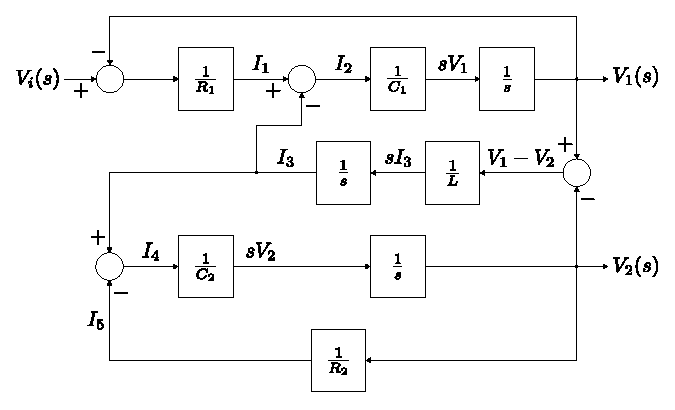
\includegraphics[scale=0.8]{cap2_fig1.eps}
	\caption{Diagrama de blocos.}
	\label{fig:exemplo1}
\end{figure}
\end{verbatim}

Este código produz a Figura~\ref{fig:exemplo1}. As figuras podem ser redimensionadas de uma forma absoluta através da opção \code{scale}, ou de forma relativa, e.g., à largura da área de texto da forma: \path{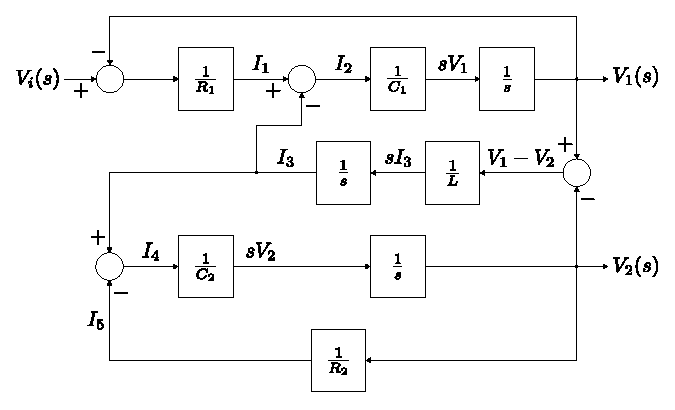
\includegraphics[width=0.5\textwidth]{cap2_fig1.eps}}. Se necessário pode também recorrer a sub-figuras (ver código deste ficheiro), como demonstrado pela Figura~\ref{fig:exemplo2} que contém as sub-figuras~\ref{fig:subfigA} e~\ref{fig:subfigB}.

\begin{figure}[htbp]
	\centering
	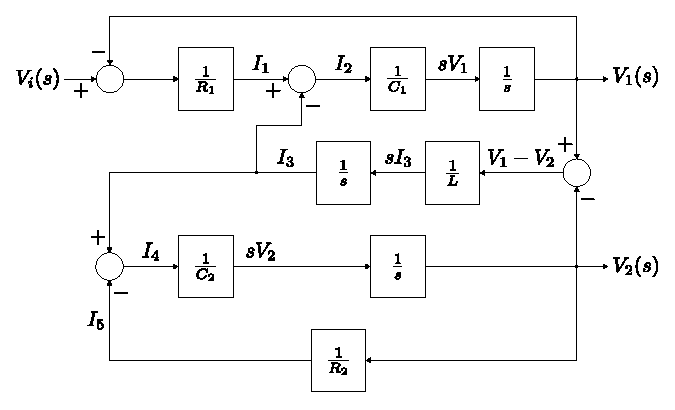
\includegraphics[scale=0.8]{cap2_fig1.eps}
	\caption{Diagrama de blocos.}
	\label{fig:exemplo1}
\end{figure}

\begin{figure}[htbp]
  \centering
  \subcaptionbox{Uma sub-figura\label{fig:subfigA}}{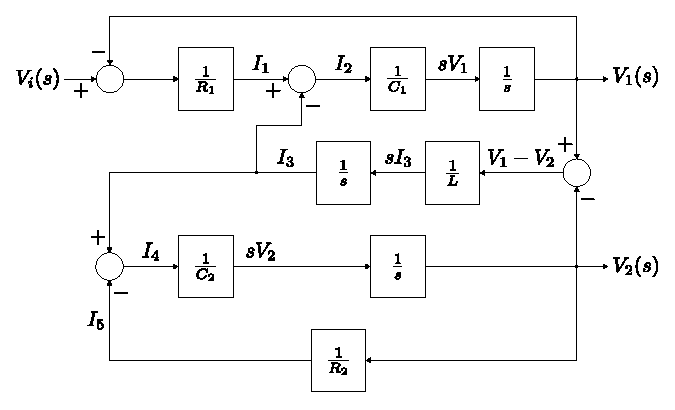
\includegraphics[width=0.45\linewidth]{cap2_fig1.eps}}
%  \hfill
  \subcaptionbox{\label{fig:subfigB}}{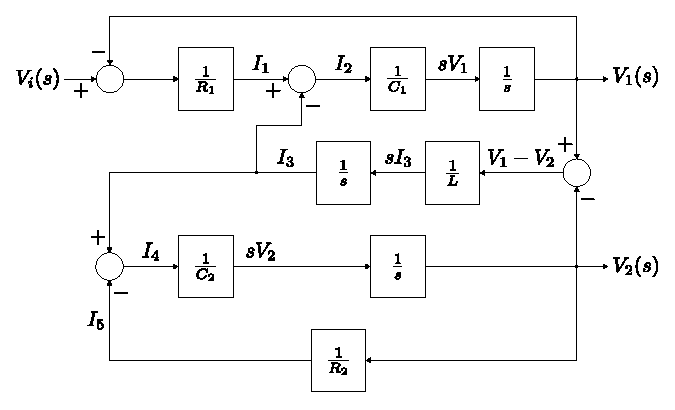
\includegraphics[width=0.45\linewidth]{cap2_fig1.eps}}
  \caption[Uma figura com duas sub-figuras.]{Uma figura com duas sub-figuras: (a) com legenda e (b) sem legenda  \cite{Motorola96}.}
  \label{fig:exemplo2}
\end{figure}

Tenha em consideração que nem sempre as figuras irão aparecer no ponto onde escreveu o código, dado que o posicionamento depende do espaço disponível na página. Posicionar as figuras é trabalho para o \LaTeX{} e por isso só se deve preocupar em fazer as imagens, de preferência em formato vetorial (e.g., EPS, PDF). Neste sentido existem várias ferramentas, sendo o Inkscape (\url{inkscape.org}) uma excelente alternativa. O \LaTeX{} por omissão aceita os formatos PDF, JPG e PNG. As figuras devem ser sempre referidas no texto e devem também ter sempre uma legenda, definida através do comando \verb|\caption{}|. Não esquecer que quando uma figura é obtida de uma referência bibliográfica, i.e., não é da sua autoria, esse facto deve ser mencionado (ver legenda da Figura~\ref{fig:exemplo2}).

Este \textit{template} disponibiliza o comando adicional \verb|\inlinegraphics| que permite inserir figuras na linha de texto. Este é um exemplo \inlinegraphics{Inlinefigureexample.png}, verifique como usar o comando no código deste ficheiro. Por vezes uma figura necessita de ser apresentada em \textit{landscape}, onde a Figura~\ref{fig:exemplo3} é um exemplo desta forma de apresentação.

%%%%%%%%%%%%%%%%%%%%%%%%%%%%%%%%%%%%

\subsection{Tabelas}

As tabelas são uma forma importante de apresentação de informação. A Tabela~\ref{tab:basictable} ilustra a aplicação das principais diretrizes a ter em consideração na construção de tabelas:

\begin{enumerate}
   \item Não usar linhas verticais.
   \item A legenda é colocada antes da tabela.
   \item Usar as macros \verb|\toprule|, \verb|\midrule| e \verb|\bottomrule| para criar as linhas horizontais, respetivamente, do topo, meio e fundo da tabela.
\end{enumerate} 

\begin{landscape}
	\begin{figure}[htbp]
		\centering
		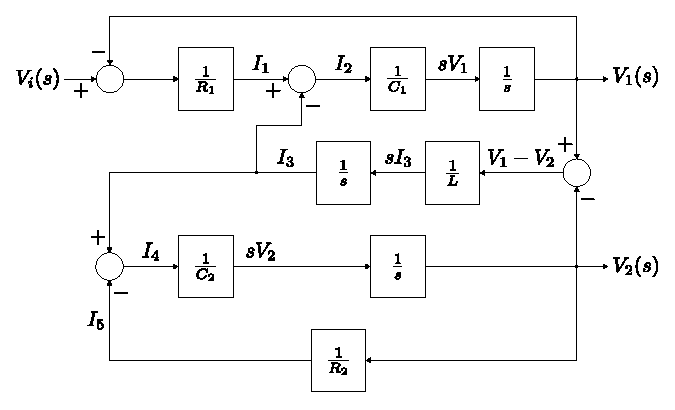
\includegraphics[scale=1.8]{cap2_fig1.eps}
		\caption{Uma figura em \textit{landscape}.}
		\label{fig:exemplo3}
	\end{figure}
\end{landscape}

Considere o seguinte código usado para criar a Tabela~\ref{tab:basictable}:

{\small
\begin{verbatim}
\begin{table}
\caption{Exemplo de uma tabela simples em \LaTeX{}.}
\label{tab:basictable}
\centering
	\begin{tabular}{l c c}
	\toprule
	\tabhead{Coluna 1} & \tabhead{Coluna 2} & \tabhead{Coluna 3} \\
	\midrule
	Linha 1 & 0.2 & 0.8\\
	Linha 2 & 0.17 & 0.7\\
	Linha 3 & 0.24 & 0.75\\
	Linha 4 & 0.68 & 0.3\\
	\bottomrule
\end{tabular}
\end{table}
\end{verbatim}
}

\begin{table}[htb]
	\caption{Exemplo de uma tabela simples em \LaTeX{}.}
	\label{tab:basictable}
	\centering
	\begin{tabular}{l c c}
	\toprule
	\tabhead{Coluna 1} & \tabhead{Coluna 2} & \tabhead{Coluna 3} \\
	\midrule
		Linha 1 & 0.2 & 0.8\\
		Linha 2 & 0.17 & 0.7\\
		Linha 3 & 0.24 & 0.75\\
		Linha 4 & 0.68 & 0.3\\
	\bottomrule
	\end{tabular}
\end{table}

Para fazer referência a tabelas use o comando \verb|\ref{<label>}|, onde  \verb|<label>| se refere ao rótulo definido por \verb|\label{<label>}|. Regra geral coloque sempre um til, i.e., \verb|Tabela~\ref{<label>}|, para introduzir um \textit{unbreakable space}. Ambientes e comandos adicionais podem ser empregues para construir tabelas mais complexas/específicas (desde que mantidas as regras gerais definidas anteriormente): \verb|tabularx|, \verb|longtable|, \verb|\multicolumn|, \verb|\multirow|, entre outros. Em caso de dificuldade na criação do código para as tabelas, sugere-se o \textit{website} \url{www.tablesgenerator.com}.

%%%%%%%%%%%%%%%%%%%%%%%%%%%%%%%%%%%%

\subsection{Listagens de código}

Para apresentar excertos de código-fonte no seu relatório este \textit{template} usa o \gls{pack} \verb|listings|. Tenha em consideração que por omissão as listagens estão definidas como flutuantes para que o \LaTeX{} as possa posicionar da melhor forma. Esta definição implica também que uma listagem não será dividida por uma nova página, pelo que é recomendado que utilize excertos que não excedam uma página. Existem muitas opções que podem ser especificadas neste ambiente, para mais informações consultar \url{en.wikibooks.org/wiki/LaTeX/Source_Code_Listings}.

O comando \verb|\printlistoflistings|, invocado no ficheiro \path{4_frontmatterlists.tex}, cria a secção ``Listagens'' no seu documento. Assim, se não necessitar de usar listagens deverá comentar este comando. A Listagem~\ref{lst:examplo1} e a Listagem~\ref{lst:examplo2} são dois exemplos de listagens de código. Analise o conteúdo deste ficheiro para mais detalhes.

\begin{center}
\begin{minipage}{0.7\linewidth}
\begin{lstlisting}[language=C, caption=Exemplo simples de C., label=lst:examplo1]
#include<stdio.h>
main()
{
	printf("Hello World");
}
\end{lstlisting}
\end{minipage}
\end{center}

Uma listagem de código também pode ser inserida diretamente de um ficheiro através do comando \verb|\lstinputlisting[<settings>]{<pathtofile>/file.c}|.

\begin{minipage}{0.9\linewidth}
\begin{lstlisting}[language=Python, caption=Exemplo longo em Python., label=lst:examplo2]
import numpy as np
    
def incmatrix(genl1,genl2):
    m = len(genl1)
    n = len(genl2)
    M = None #to become the incidence matrix
    VT = np.zeros((n*m,1), int)  #dummy variable
    
    #compute the bitwise xor matrix
    M1 = bitxormatrix(genl1)
    M2 = np.triu(bitxormatrix(genl2),1) 

    for i in range(m-1):
        for j in range(i+1, m):
            [r,c] = np.where(M2 == M1[i,j])
            for k in range(len(r)):
                VT[(i)*n + r[k]] = 1;
                VT[(i)*n + c[k]] = 1;
                VT[(j)*n + r[k]] = 1;
                VT[(j)*n + c[k]] = 1;
                
                if M is None:
                    M = np.copy(VT)
                else:
                    M = np.concatenate((M, VT), 1)               
                VT = np.zeros((n*m,1), int)  
    return M
\end{lstlisting}
\end{minipage}

%%%%%%%%%%%%%%%%%%%%%%%%%%%%%%%%%%%%

\subsection{Equações}

Se a sua tese fizer uso de conteúdo matemático, então a opção de usar o \LaTeX{} foi a mais acertada. O livro ``Uma não tão pequena introdução ao \LaTeX{}'' tem informação suficiente para a maioria dos casos de composição matemática, mas para conteúdos mais completos recomenda-se o guia \url{tug.ctan.org/info/short-math-guide/short-math-guide.pdf}. Adicionalmente, uma extensa lista de símbolos pode ser consultada em \url{tug.ctan.org/info/symbols/comprehensive/symbols-a4.pdf}.

O \LaTeX{} permite a escrita de equações \textit{inline} como $E = mc^{2}$ ou em modo \textit{display}, sendo neste caso  automaticamente numeradas:

\begin{verbatim}
\begin{equation}
	E = mc^{2} .
	\label{eqn:einstein}
\end{equation}
\end{verbatim}

\noindent que produz a famosa equação:

\begin{equation}
E = mc^{2} .
\label{eqn:einstein}
\end{equation}

Alternativamente, se pretender que (\ref{eqn:einstein}) não seja numerada pode usar o código \verb|$$ E = mc^{2} $$| que produz:
$$ E = mc^{2} .$$

%%%%%%%%%%%%%%%%%%%%%%%%%%%%%%%%%%%%

\subsection{Teoremas}

Teoremas, lemas e corolários devem ser numerados por ordem crescente. O \textit{template} fornece estes ambientes adaptados ao idioma selecionado para o documento em \file{main.tex}. Através do comando \verb|\newtheorem| pode criar ambientes adicionais do mesmo tipo (no ficheiro \file{preamble.tex}). 

\begin{theorem}
Isto é um exemplo da aplicação do ambiente \code{theorem}. Os teoremas são numerados por ordem crescente, iniciando em 1.
\end{theorem}

\begin{corollary}
Isto é um exemplo da aplicação do ambiente \code{corollary}. Os corolários são numerados por ordem crescente, iniciando em 1.
\end{corollary}

\begin{lemma}
Isto é um exemplo da aplicação do ambiente \code{lemma}. Os lemas são numerados por ordem crescente, iniciando em 1.
\end{lemma}

%%%%%%%%%%%%%%%%%%%%%%%%%%%%%%%%%%%%
\clearpage
\section{Notas Adicionais}

\textbf{Boa sorte!}

